\cleartooddpage[\thispagestyle{empty}]
\chapter{Analysis}

\section{Veritas Data}
  The analysis in this thesis relies on three sets of VERITAS data.
  One set observes the Crab Nebula, another observed the Galactic Center, and a third set observes a dark region \SI{5}{\degree} NW of the Galactic Center.
  This dark region is referred to as  Sgr A* Off, and is located at (l,b)=(357.3396\degree, 3.9984\degree, shown in Figure \ref{fig:gcfieldsofview}.

  \begin{figure}[ht]
    \begin{center}
      \includegraphics[width=0.95\textwidth]{images/skypointings/plot.eps}
      \caption[VERITAS Galactic Center Pointings]{Fields of view for Galactic Center observations.}\label{fig:gcfieldsofview}
    \end{center}
  \end{figure}

  All three sets of data include observations from both the V5 epoch (after moving T4 but before the camera upgrade), and the V6 epoch (after the camera upgrade).
  All used data was taken from April 2010 to June 2016.

  %
  % times calculated with $VERIPY/thesis/plots/obs_times.py
  %
  \begin{table}[]
    \centering
    \caption{Hours of observations taken at each source/epoch combination.}
    \label{my-label}
    \begin{tabular}{|l|l|l|l|}
      \hline
      \textbf{Epoch} & \textbf{Crab} & \textbf{Sgr A*} & \textbf{Sgr A* Off} \\ \hline
      V5             & 3.3           & 39.8            & 8.0                 \\ \hline
      V6             & 5.5           & 55.4            & 4.1                 \\ \hline
    \end{tabular}
  \end{table}


  \begin{figure}[ht]
    \centering
    \includegraphics[width=0.95\textwidth]{data_elevation_plots/plot.eps}
    \caption[VERITAS Data Elevation Exposure]
    {Camera center elevation for the three sets of data. (Update this plot!!??)}
    \label{fig:datapointingelevations}
  \end{figure}

  There are comparativly fewer Sgr A* Off observations, as there are no gamma-ray emitters at or near that position, and telescope time is valuable.
  There is also even fewer Crab observations, as the majority of its observations are done at higher elevations, where the telescope is more sensitive to lower energies.
  
  For all of these observations, quality checks were applied.
  This includes monitoring the telescope hardware and weather by a team of VERITAS collaboration members who take the observations.
  After the data is taken, a separate collaboration member will go through each observation to check it again, and mark any bad observations or apply time cuts, which are then removed.

  As multiple studies in the past have shown that the different VERITAS epochs perform differently, each epoch has their own separate set of effective areas, point spread functions, energy migration matricies, and camera background models.
  In addition, specific IRFs were calculated for additional data dimensions, including the frequency of night sky background photons in the camera, the telescope elevation, the event energy, and each event's distance from the camera center.

\section{Likelihood Ratio Test}
  The likelihood ratio test useful for comparing two hypotheses.
  They are referred to as the null and alternative hypotheses.
  Each hypothesis consists of a predicted number of events at each point in the energy/space/time parameter space.
  Once each hypothesis is constructed, the likelihood for each can be computed.
  The ratio of the two likelihoods then follows a gaussian (with certain assumptions), meaning the sigificance of the alternative hypothesis over the null can be calculated.

  As part of this likelihood ratio test, the signal and background models must be constructed.
  Background models can be camera background models (discussed in section \ref{sec:bkgmodels}), or astrophysical models of background gamma-ray emitters.
  In this context, the null hypothesis consists of only background models, while the alternative hypothesis consists of all the background models plus one signal model.

\section{Background Models}\label{sec:bkgmodels}
  The background models predict the amount of background counts produced by a gamma-ray-empty sky.
  This is used to model the effect of the background (primarily proton) events, which are several orders of magnitude more populous than the gamma rays.
  Producing the backgrounds is performed by binning observation sources with weak or no gamma-ray emission.
  For this low-elevation analysis, special observation runs were taken several degrees away from the galactic center.

  (skymap of GC and GC Off runs??)

  These background runs were then assembled into background models via the procedure in \ref{background_production}.
  To account for the difference between the V5 and V6 observatory configurations, the background observations are divided up based on their epoch, producing unqiue backgrounds for each epoch.
  Built into this procedure is that the background values vary as a function of distance from the camera center, and the event energy.

  It should be noted that CTOOLS backgrounds are in RA/DEC detector coordinates, instead of Az/El detector coordinates. (??)

  To confirm that these background models fit properly, a simple likelihood analysis was performed with the Off observations and their backgrounds.
  If the background models were assembled astutely, after the liklelihood normalization, the number of events observed and predicted by the models is shown in figure ??.

  (using just the background observations, show profile plots in galactic-b and energy??)

\section{Test Point Sources}
  To verify that the CTOOLs likelihood analysis is working properly, two point sources were analyzed first, before any dark matter analysis was performed.
  The first was on the well-studied Crab nebula, and the second was on the source at the center of our galaxy.
  To also uncover any low-elevation effects, the Crab observations were limited to ones with elevations < \SI{32.5}{\degree}.

  (plot of Crab, Sgr A*, Sgr A* Off sources elevations??)

  \subsection{Test Crab Analysis}

    In order to test that the converted data, irfs, and ctools likelihood engine all work properly, a test analysis on the Crab nebula was performed.
    As the Crab nebula is the brightest gamma ray emitter in the sky, it has been observed extensively by VERITAS and other gamma ray telescopes.
    Since the Galactic Center only rises to around 30\degree elevation, elevation effects would also need to be searched for.
    After searching for low-elevation Crab observations, a total of 17.1 hours of livetime were found.
    These consist of 7.3(doesn't match with plot??) hours of V5 epoch data, and 9.8(doesn't match with plot??) hours of V6 epoch data.
    
    \begin{figure}[h]
      \centering
      \includegraphics[width=0.95\textwidth]{images/test_crab_analysis/plot_elev27_5_32_5deg_4_70TeV_wobbleall_Epochall_skymap.eps}
      \caption[Crab Counts Skymap]
      {
        Skymap of event positions.
        No corrections are made for observing time or effective area.
        Observation time is different??
      }
      \label{fig:crab_skymap}
    \end{figure}
    
    The Crab was modeled by a single point source with a simple power law spectrum:

    \begin{equation} \label{eqn:powerlaw}
    F\left( E \right) = I_{0} \left( \frac{E}{E_{0}} \right)^{-\gamma}
    \end{equation}

    Only events between 4 and 70 TeV are used in this test analysis.
    At an elevation of 25\degree, the reconstruction software is able to reconstruct events as low as 1.5 TeV.
    But, in this 'threshold' energy region, the camera sensitivity starts to decrease in a poorly understood way, and IRFs in this region are not accurate.
    Part of this decrease is explored in section (see figures \ref{fig:bkgvsel_crab} and \ref{fig:bkgvsel_sgra}), but implementing corrections requires large changes to existing code, along with a larger set of simulations, neither of which were feasible during this work.
    Above 70 TeV, simulations become too computationally expensive to create when attempting to calculate IRFs.
    
    After fitting all events from \SI{4}{TeV} to \SI{70}{TeV}, with a pivot energy $ E_{0}= \SI{10}{TeV} $, the $ I_{0} = \left(1.472\pm0.09\right)*10^{-19} \frac{ph}{cm^{2} s MeV} $, $ \gamma = 2.382 \pm 0.076 $, with a Test Statistic of 1929.01. (?? update values!).
    As the crab (alternative) hypothesis has 110 free parameters, and the no-crab (null) hypothesis has 108 free parameters, the Test Statistic has $ 110 - 108 = 2 $ degrees of freedom.
    This is equivalent to a significance of ??.
    
    
    \begin{figure}[h]
      \centering
      \includegraphics[width=0.95\textwidth]{images/test_crab_analysis/plot_elev27_5_32_5deg_4_70TeV_wobbleall_Epochall.eps}
      \caption[Crab Test Spectrum]
      {
        Crab spectra from various analyses and observatories.
        Red is the spectra from the CTOOLS analysis described in this chapter.
        Blue is the standard VERITAS Event Display spectrum using the same set of observations.
      }
      \label{fig:crab_test_spectra}
    \end{figure}
    
    In figure \ref{fig:crab_test_spectra}, the fitted crab spectra is shown, along with literature results from earlier VERITAS, HESS, and MAGIC observations of the Crab.
    
    \begin{figure}[h]
      \centering
      \includegraphics[width=0.95\textwidth]{images/test_crab_analysis/plot_elev27_5_32_5deg_4_70TeV_wobbleall_Epochall_spl.eps}
      \caption[Crab Profile along Galactic L]
      {
        The number of counts along a 0.16\degree-wide-slice through the Crab along the Galactic L axis.
        Blue is the number of observed counts.
        Green is the number of counts predicted by the models.
        Purple is the number of counts predicted by only the camera-background models.
      }
      \label{fig:crab_profile_l}
    \end{figure}

    \begin{figure}[h]
      \centering
      \includegraphics[width=0.95\textwidth]{images/test_crab_analysis/plot_elev27_5_32_5deg_4_70TeV_wobbleall_Epochall_spb.eps}
      \caption[Crab Profile along Galactic B]
      {
        The number of counts along a 0.16\degree-wide-slice through the Crab along the Galact B axis.
        Blue is the number of observed counts.
        Green is the number of counts predicted by the models.
        Purple is the number of counts predicted by only the camera-background models.
      }
      \label{fig:crab_profile_b}
    \end{figure}
    
    \begin{figure}[h]
      \centering
      \includegraphics[width=0.95\textwidth]{images/test_crab_analysis/plot_elev27_5_32_5deg_4_70TeV_wobbleall_Epochall_splalt.eps}
      \caption[Crab Profile along Galactic L Off Source]
      {
        The number of counts along a 0.16\degree-wide-slice along the Galactic L axis.
        Blue is the number of observed counts.
        Green is the number of counts predicted by the models.
        Purple is the number of counts predicted by only the camera-background models.
        This slice doesn't go through the Crab, but instead 1\degree higher in Galactic B.
        As this doesn't include the Crab, this plot primarily demonstrates the camera background modelling.
      }
      \label{fig:crab_profile_l_off}
    \end{figure}

    \begin{figure}[h]
      \centering
      \includegraphics[width=0.95\textwidth]{images/test_crab_analysis/plot_elev27_5_32_5deg_4_70TeV_wobbleall_Epochall_ep.eps}
      \caption[Crab Profile in Energy]
      {
        The number of counts in a 0.6\degree x 0.6\degree square centered on the Crab, vs energy.
        Blue is the number of observed counts.
        Green is the number of counts predicted by the models.
        Purple is the number of counts predicted by only the camera-background models.
      }
      \label{fig:crab_profile_energy}
    \end{figure}
    
    The fitted models can also be viewed, as a check that the likelihood engine is fitting the models to the data.
    In figure \ref{crab_skymap}, the position of all counts is shown in galactic l and b.
    In figures \ref{fig:crab_profile_l} and \ref{fig:crab_profile_b}, the counts in the observations and models were integrated along a slice of galactic l and b.
    The counts from only the camera background models is shown, along with the counts from all camera backgrounds plus the point source.
    The difference between these two lines is then the counts from the Crab point source model.
    In figure \ref{fig:crab_profile_energy}, a similar plot is made, though integrated in a \SI{0.6}{\degree}x\SI{0.6}{\degree} square around the crab at different energies.

\section{Dark Matter Likelihood Analysis}

  \subsection{Non-Dark-Matter Models}
  For this analysis, a point source model was added at the position of Sgr A*.
  This is because other analyses (cite??) have indicated that the bright gamma-ray source at Sgr A* is not best modeled by a dark matter halo.
  % DM is unlikely to be the cause of the point source in the GC
  % Updated cosmic-ray and radio constraints on light dark matter: Implications for the GeV gamma-ray excess at the Galactic Center
  % Bringmann 2014
  % https://journals.aps.org/prd/pdf/10.1103/PhysRevD.90.123001
  Instead, a point source with a broken power law spectrum (Equation \ref{eqn:brokenplaw}) is added to the list of models, with the magnitude of its flux left free by the likelihood engine.
  
  \begin{equation}\label{eqn:brokenplaw}
    \frac{dN}{dE} = N_{0} * { \left ( \frac{E}{E_{pivot}} \right ) }^{\alpha} {e}^{-\frac{E}{E_{cut}}}
  \end{equation}
  
  From \cite{VeritasGCRidge2015}, the specific values used in this point source were $E_{pivot}=\SI{1}{TeV}$, $E_{cut}=\SI{12.8}{TeV}$, and $\alpha=-2.1$.
  The normalization $N_{0}$ was initially set to $2.8*{10}^{-12}\,\text{cm}^{-2}\,\text{s}^{-1}\,\text{TeV}^{-1}$, but was left free in the likelihood optimization, while $E_{pivot}$, $E_{cut}$, and $\alpha$ were all fixed.
  The normalization was left free to allow for the potential of some mixing between the point source events and any dark matter halo events, i.e. a stronger dark matter halo gamma-ray flux would result in a weaker point source flux.
  
  Diffuse emission, eliminated due to complexity?

  \subsection{Dark Matter Models}
  Dark Matter halos are modeled by a spherically-symmetric mass-per-volume density profile.
  In this analysis, an Einasto density profile (discussed in section \ref{dm_spatial}) is used as the spatial component of the dark matter halo model.
  For the spectral component, each dark matter mass tested has its own spectrum produced with clumpy, which is based on ?? (see section \ref{dm_spectral}).

  \subsection{Likelihood Results}
  
  \begin{figure}[ht]
    \begin{center}
      \includegraphics[width=0.95\textwidth]{images/likelihood_analysis/counts_skymap.eps}
      \caption[Galactic Center Counts Skymap]{Skymap of all event positions used in this analysis.  No adjustment for effective area, observation time, or background rate is done here.}\label{fig:gc_counts_skymap}
    \end{center}
  \end{figure}

  \begin{figure}[ht]
    \begin{center}
      \includegraphics[width=0.95\textwidth]{images/likelihood_analysis/counts_enhist.eps}
      \caption[Galactic Center Counts Energy Histogram]{Histogram of all event positions used in this analysis.  No adjustment for effective area, observation time, or background rate is done here.}\label{fig:gc_counts_enhist}
    \end{center}
  \end{figure}

  The analysis uses the $b\bar{b}$ annihilation channel, and are shown for just at $10\text{TeV}$.
  
  \begin{figure}[ht]
    \begin{center}
      \includegraphics[width=0.95\textwidth]{images/likelihood_analysis/profile_gal_l.eps}
      \caption[Galactic Center Profile vs Galactic L]{Observed vs modeled counts in a slice of the sky parallel to the galactic L axis at $B=0$.  Modeled counts from camera-background-models are shown in purple, total modeled counts are shown in green.  The feature where the observed counts are shifted to the left of the models is likely due to unaccounted-for elevation effects in the camera background models.}\label{fig:gc_profile_gal_l}
    \end{center}
  \end{figure}

  \begin{figure}[ht]
    \begin{center}
      \includegraphics[width=0.95\textwidth]{images/likelihood_analysis/profile_gal_b.eps}
      \caption[Galactic Center Profile vs Galactic B]{Observed vs modeled counts in a slice of the sky parallel to the galactic B axis at $L=0$.  Modeled counts from camera-background-models are shown in purple, total modeled counts are shown in green.  The feature where the observed counts are shifted to the left of the models is likely due to unaccounted-for elevation effects in the camera background models.}\label{fig:gc_profile_gal_b}
    \end{center}
  \end{figure}

  \begin{figure}[ht]
    \begin{center}
      \includegraphics[width=0.95\textwidth]{images/likelihood_analysis/profile_energy.eps}
      \caption[Galactic Center Profile vs Energy]{Observed vs modeled counts in a ${0.2}^{\circ}\times{0.2}^{\circ}$ square bin centered on Sgr A*.  Modeled counts from camera-background-models are shown in purple, total modeled counts are shown in green.}\label{fig:gc_profile_energy}
    \end{center}
  \end{figure}
  
  
\section{Upper Limit}
  An upper limit on the flux of a source can be calculated by scaling the flux of a model until the log-likelihood is at the 0.95 confidence level.
  This is done by using the ctulimit tool in ctools.
  
  Then from the dark matter flux equation ??, an upper limit on the observed gamma-ray flux can be used to calculate an upper limit on the velocity-averaged crosssection.
  
  \begin{equation}\label{eqn:ulim}
    \frac{d\phi}{dE d\omega} = \frac{ \sigma v (fixme!??)}{8\pi m_{\chi}^{2}} \frac{dN_{\gamma}}{dE} \int \rho^{2} dl
  \end{equation}
  
  Since, when all other variables are fixed, a larger gamma ray flux results from a larger velocity-averaged crosssection, they can both be replaced with their upper limits (??).

  \begin{figure}[ht]
    \begin{center}
      \includegraphics[width=0.95\textwidth]{images/ulimit/final_upper_limit_plot.eps}
      \caption[Dark Matter Upper Limit Plot]{Dark Matter upper limits on velocity-averaged cross-sections.}\label{fig:ulim}
    \end{center}
  \end{figure}
  
  
